
\فصل{مقدمه}

در این فصل مسئله‌ی اصلی پژوهش، یعنی امتیاز ،ASPECT به طور دقیق‌تر مورد بررسی قرار می‌گیرد و علت اهمیت بالای آن در زمینه‌ی سکته‌ی مغزی عنوان می‌شود.
سپس بررسی می‌شود که آیا این مسئله در پژوهش‌ها و محصولات مرتبط، حل شده‌است یا خیر و اینکه پژوهش حاضر چه مزیتی در این حوزه به همراه خواهد داشت.
در پایان نیز ساختار کلی پایان‌نامه شرح داده می‌شود.

\قسمت{تعریف مسئله}

سکته‌ی مغزی یکی از علل مهم مرگ ومیر و ناتوانی‌های اکتسابی در جهان است.
%Donkor, E.S., 2018. Stroke in the century: a snapshot of the burden, epidemiology, and quality of life. Stroke research and treatment, 2018.
امروزه روش‌های درمانی مختلفی برای بیماران مبتلا به این عارضه وجود دارد.
اما تجویز روش درمانی مناسب، برای هر بیمار، با توجه به وضعیت وی، متفاوت است.
در واقع لازم است که متخصصان، ملاک و معیاری از وضعیت پیشرفت و وخامت سکته داشته باشند تا بتوانند یک روش درمانی را برای بیمار، مناسب یا نامناسب قلمداد کنند.
یکی از مهم‌ترین این معیارها، امتیاز ASPECT است.\\

\lr{The Alberta Stroke Program Early CT Score (ASPECTS)} یک امتیاز از ۱ تا ۱۰ است که معیاری از وخامت سکته در بیمار را به دست می‌دهد.
درواقع این امتیاز از بررسی وضعیت ۱۰ ناحیه‌ی مغزی ،که در دو نیم‌کره‌ی مغز به صورت متقارن وجود دارند، محاسبه می‌شود.
شکل ~\ref{fig:aspects-regions} این ۱۰ ناحیه را نشان می‌دهد.
در صورتی که هیچ عارضه‌ی انسدادی در مغز وجود نداشته باشد، امتیاز ASPECT برابر ۱۰ خواهد بود و به ازای هر ناحیه‌ای که آسیب دیده‌است، یک امتیاز از ۱۰ کم می‌شود.
به این ترتیب بیماری که هر ۱۰ ناحیه‌ی ASPECTS او، حداقل در یک نیم‌کره، آسیب دیده‌باشد، امتیاز صفر را دریافت خواهد کرد.

\begin{figure}[ht]
    \centering
    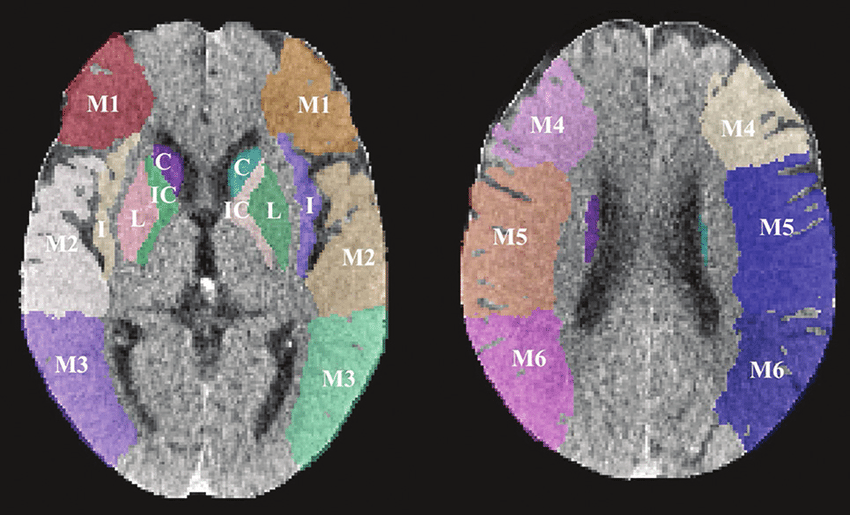
\includegraphics[width=\textwidth, keepaspectratio]{aspects-regions.png}
    \caption[]{نواحی ASPECTS در دو برش از مغز. ۱۰ ناحیه شامل ،I ،C ،L ،IC \lr{M6}-\lr{M1}.}
    \label{fig:aspects-regions}
\end{figure}
%Kuang, Hulin & Najm, Mohamed & Chakraborty, Debabrata & Maraj, Nicholas & Sohn, Sung-Il & Goyal, Mayank & Hill, Michael & Demchuk, Andrew & Menon, Bijoy & Qiu, Wu. (2018). Automated ASPECTS on Non-Contrast CT Scans in Acute Ischemic Stroke Patients Using Machine Learning. American Journal of Neuroradiology. 10.3174/ajnr.A5889. 


این امتیاز سپس می‌تواند معیاری در اختیار متخصصان قرار دهد که تشخیص بدهند آیا لخته‌زدایی مکانیکی
\footnote{\lr{Mechanical Thrombectomy}}
برای بیمار مناسب است یا خیر.
یه عنوان مثال، ممکن است در یک سیاست تصمیم‌گیری، بیمارانی که امتیاز بیشتر/مساوی ۶ را کسب کرده‌اند، برای لخته‌زدایی مکانیکی، مناسب تشخیص داده‌شوند.
% Seyedsaadat, S.M., Neuhaus, A.A., Nicholson, P.J., Polley, E.C., Hilditch, C.A., Mihal, D.C., Krings, T., Benson, J., Mark, I., Kallmes, D.F. and Brinjikji, W., 2021. Differential contribution of ASPECTS regions to clinical outcome after thrombectomy for acute ischemic stroke. American Journal of Neuroradiology, 42(6), pp.1104-1108.
به این نوع از امتیازدهی که وضعیت بیماران را به دو دسته‌ی بالا و پایین یک آستانه تقسیم می‌کنند، امتیاز دوبخشی‌شده‌ی ASPECTS می‌گویند.
درواقع در اکثر موارد، تشخیص درمان لخته‌زدایی به کمک همین حد آستانه بر روی امتیاز ASPECTS انجام می‌شود و از این جهت، به امتیاز‌دهی دوبخشی اهمیت بیشتری می‌بخشد.\\

نکته‌ی حائز اهمیت آن است که امتیازدهی ،ASPECT حتی برای متخصصین این حوزه، یک امر چالش‌بر‌انگیز است.
به نحوی که در یک مطالعه،
%van Horn, N., Kniep, H., Broocks, G., Meyer, L., Flottmann, F., Bechstein, M., Götz, J., Thomalla, G., Bendszus, M., Bonekamp, S. and Pfaff, J.A.R., 2021. ASPECTS interobserver agreement of 100 investigators from the TENSION study. Clinical Neuroradiology, pp.1-8.
میزان توافق میان امتیازدهندگان، تنها ۲۸٪ محاسبه شده‌است.
از طرفی، نشان داده شده‌است که ابزار‌های محاسبه‌ی خودکار ،ASPECT می‌توانند
میزان این توافق و سرعت امتیازدهی متخصصان را افزایش دهند.
%Chen, W., Wu, J., Wei, R., Wu, S., Xia, C., Wang, D., Liu, D., Zheng, L., Zou, T., Li, R. and Qi, X., 2022. Improving the diagnosis of acute ischemic stroke on non-contrast CT using deep learning: a multicenter study. Insights into Imaging, 13(1), pp.1-12.
به همین جهت، این پژوهش قصد دارد با ارائه‌ی یک روش خودکار تشخیص امتیاز دوبخشی ASPECT 
در راستای این بهبود دقت و سرعت، راهگشا باشد.

\قسمت{اهمیت موضوع}
میان دقت، سرعت و دسترس‌پذیری در تشخیص سکته‌ی مغزی، یک بده‌بستان
\footnote{tradeoff}
وجود دارد.
یک‌سری تصاویر مانند ،MRI علائم سکته را بهتر در خود نمایان کرده و تشخیص را برای متخصصان ساده‌تر می‌کنند.
اما اخذ این تصاویر، زمان زیادی نیاز دارد و ممکن است در تمام مراکز تصویر‌برداری نیز در دسترس نباشند.
از سوی دیگر، تصاویر ،CT علائم سکته را کمتر مشخص می‌کنند و باعث می‌شوند که تشخیص، سخت‌تر و توافق میان تشخیص‌دهندگان کمتر شود.
اما مزیت این مدل تصویربرداری، در سرعت اخذ تصویر و کاربرد فراگیر آن در اکثر ماکز تصویر برداری است.\\
اصطلاحی در این حوزه وجود دارد که عنوان می‌کند "زمان، مغز است". 
%Saver, J.L., 2006. Time is brain—quantified. Stroke, 37(1), pp.263-266.
این جمله به اهمیت زمان و لزوم تشخیص و درمان سریع سکته‌ی مغزی اشاره می‌کند.
به طور متوسط، در بیمارانی که دچار سکته‌ی مغزی انسدادی شده‌اند، در هر دقیقه، ۱.۹ میلیون سلول عصبی از بین می‌رود.
این عدد در مقایسه با نرخ عادی از بین رفتن سلول‌های عصبی، مانند آن است که مغز در یک ساعت، به مدت ۳.۶ سال عمر کرده‌است.
%همان
به همین جهت، سرعت عمل در تشخیص سکته‌ی مغزی و آغاز هر چه زودتر درمان آن، امری حیاتی است.
در نتیجه در بده‌بستان میان دقت و سرعت، این سرعت است که برتری می‌یابد و تصویربرداری CT و روش‌های تشخیصی مبتنی بر آن را غالب می‌کند.\\
امتیازدهی ASPECT یک روش تشخیصی مبتنی بر CT است.
به همین دلیل است که پژوهش حول این مسئله، از اهمیت بالایی برخوردار است.
اما همانطور که پیش‌تر ذکر شد، علی‌رغم سرعت بالای تشخیص در این روش، افزایش دقت حاصل از آن، یک موضوع چالش برانگیز است.
عدم توافق بالا میان تشخیص متخصصان نیز خبر از این مشکل دارد.
مشکلی که همچنان میان متخصصان انسانی ماندگار است.
هوش مصنوعی و روش‌های یادگیری ماشین می‌توانند به حل این مشکل کمک کنند.
پژوهش‌هایی انجام شده‌است
%Chen, W., Wu, J., Wei, R., Wu, S., Xia, C., Wang, D., Liu, D., Zheng, L., Zou, T., Li, R. and Qi, X., 2022. Improving the diagnosis of acute ischemic stroke on non-contrast CT using deep learning: a multicenter study. Insights into Imaging, 13(1), pp.1-12.
که نشان می‌دهد تشخیص خودکار امتیاز ASPECT می‌تواند توافق میان متخصصان را افزایش بدهد.
بنابراین ضروری است که این روش‌ها، با افزایش هرچه بیش‌تر دقت، در راستای بهبود سرعت و دقت خدمات درمانی سکته‌ی مغزی، کمک‌کننده باشند.

\قسمت{ادبیات موضوع}

فعالیت‌هایی که به طور مستقیم در حوزه‌ی امتیازدهی ASPECT انجام می‌شوند را می‌توان در دو دسته‌ی کلی بررسی کرد.
دسته‌ی اول، برنامه‌های کاربردی
\footnote{Application} ‌هایی هستند 
که به صورت تجاری عرضه شده و در حال استفاده در مراکز درمانی می‌باشند.
از جمله‌ی این برنامه‌ها می‌توان به ،RapidAI Viz.ai و e-ASPECTS اشاره کرد.
بعضاً این برنامه‌ها بر روی چندین میلیون تصویر از بیش از ۱۰۰ کشور دنیا آموزش دیده‌اند
% https://www.rapidai.com/
و به دقت بسیار مطلوبی دست یافته‌اند.\\
دسته‌ی دوم شامل پژوهش‌هایی می‌شود که بر روی
تعداد تصاویر
های بسیار کوچک‌تری کار می‌کنند.
مجموعه‌داده‌
\footnote{dataset}
ای که محدود به یک یا چند مرکز درمانی می‌شوند و از نظر تنوع و تعداد،‌ با برنامه‌های فوق‌الذکر قابل مقایسه نیستند.
این پژوهش‌ها سعی دارند روش‌های جدید برای تشخیص ASPECTS ارائه دهند و یا توانایی مدل‌های یادگیری پیشین را بر روی مسئله‌ی ASPECTS بررسی کنند.
 این مطالعات و پژوهش‌های انجام‌شده، هر یک با در نظر 
 گرفتن محدودیت‌های  موجود، مورد ارزیابی قرار 
 می‌گیرند.
روش‌های پیش‌رو، سپس می‌توانند در هسته‌ی محاسباتی برنامه‌های تجاری قرار بگیرند 
و با استفاده از ظرفیت‌های داده‌ای و محاسباتی موجود، نتایج بهتری را ارائه دهند.\\
بنابراین، دو دسته فعالیتی که در حوزه‌ی ASPECTS معرفی شد، یعنی برنامه‌های کاربردی توانمند و فعالیت‌های پژوهشی، هر دو نیاز هستند و به نحوی مکمل هم می‌باشند.
بدیهی‌ است که پژوهش حاضر، در دسته‌ی دوم این فعالیت‌ها قرار می‌گیرد
و در ادامه‌ی این نوشتار نیز، تنها پژوهش‌های مطالعاتی انجام شده در حوزه‌ی ASPECTS مورد بررسی، ارجاع و مقایسه قرار خواهند گرفت.
در فصل سوم، این پژوهش‌ها به تفصیل بیشتری مورد 
بحث قرار می‌‌گیرند و
محدودیت‌ها و مزیت‌های هر یک بررسی می‌شود.
به طور کلی، کار‌های پیشین از نظر میزان داده‌ی موجود، نوع اطلاعات برچسب
\footnote{label}
داده‌ها،
نوع اطلاعات خروجی و
\dots 
قابل دسته‌بندی و مقایسه هستند.
در بخش سوم ذکر خواهد شد که پژوهش حاضر، یکی از معدود مطالعاتی است که با محدودیت‌های داده‌ای مشابه انجام شده‌است و 
در این زمینه به نتایج بسیار مطلوبی دست یافته‌است.

\قسمت{اهداف پژوهش}

% تصاویر موجود در مراکز تصویربرداری مختلف در برخی جزئیات با هم تفاوت دارند.
% همچنین ترکیب جمعتی هر مجموعه، منحصر به همان مجموعه است و تابعی از میانگین سن، جنسیت، وضعیت عمومی سلامت و \dots همان 
% منطقه می‌باشد.
% به همین جهت، 
% روش‌های ارائه شده بر روی یک مجموعه‌داده‌ی محدود، ممکن است بر روی یک مجموعه‌داده‌ی دیگر، به نتایج مشابهی دست‌نیابد.
پیش‌تر ذکر شد که محدودیت‌های داده‌ای، تاثیر به‌سزایی در توانایی و عملکرد روش‌های یادگیری ماشین دارند.
یکی از مهم‌ترین چالش‌های حوزه‌ی یادگیری ماشین نیز در کسب بهترین نتایج از داده‌های محدود-چه از نظر کمی و چه از نظر کیفی- می‌باشد.
از طرفی فراهم کردن مجموعه‌داده‌های بزرگی که توسط متخصصان به صورت جزئی برچسب‌گذاری شده‌باشند، امری دشوار، زمان‌بر و گاه غیر عملی است.
بنابراین، ارائه‌ی روش‌هایی که بتوانند از حداکثر قابلیت‌های چنین مجموعه‌داده‌هایی استفاده کنند از اهمیت بالایی برخوردار است.
این پژوهش در وهله‌ی اول می‌کوشد تا طرفیت موجود در داده‌های مراکز درمانی کشور را در زمینه‌ی تشخیص سکته‌ی مغزی بسنجد و سپس روش کارآمد و تکرارپذیری را در حوزه‌ی یادگیری تصاویر پزشکی، به طور خاص محاسبه‌ی ،ASPECT ارائه کند.
این روش علی‌رغم محدودیت‌های موجود، به عملکرد قابل مقایسه‌ای با کارهای مشابه دست یافته‌است و
به علت جامعیت بالا، با تنظیمات جزئی، قابل اعمال بر روی سایر کاربرد‌های پزشکی می‌باشد.


\قسمت{ساختار پایان‌نامه}

این پایان‌نامه در شش فصل به شرح زیر ارائه می‌شود.
برخی مفاهیم اولیه در رابطه با سکته‌ی مغزی انسدادی و امتیاز ASPECT در بخش دوم به اختصار اشاره شده‌است.
این مفاهیم از آن جهت اهمیت دارند که انطباق ساختار مدل ارائه شده با روش های مورد استفاده‌ی متخصصان را بهتر مشخص می‌کند.
همچنین در درک روش‌های مختلف ارائه‌شده در کارهای پیشین و نیامندی‌های داده‌ای هر یک راهگشا خواهد بود.
فصل سوم به مطالعه و بررسی کارهای پیشین مرتبط با امتیاز‌دهی خودکار ASPECT می‌پردازد.
در فصل چهارم، روش مورد استفاده در پژوهش حاضر شرح داده می‌شود 
و در بخش پنجم، نتایج حاصله از این روش عنوان می‌شوند.
در نهایت،‌ فصل ششم به جمع‌بندی کارهای انجام شده، موفقیت‌ها و ناکارآمدی‌های متصور برای این پژوهش و ارائه‌ی پیشنهادهایی برای انجام کارهای آتی خواهد پرداخت.